\documentclass{article}
\usepackage{amsmath}
\usepackage{amssymb}
\usepackage{tikz}
\usepackage{float}
\usepackage{subcaption}

\begin{document}

\textbf{EXAMPLE 1.} Three balls are drawn at random without replacement from a box containing 3 white, 2 red and 3 black balls. If $X$ denotes the number of white balls drawn and $Y$ denotes the number of red balls drawn, find the joint probability distribution of $(X,Y)$.

\textbf{Solution.} The total number of balls is $3 + 2 + 3 = 8$. Since 3 balls are drawn without replacement, the total number of possible outcomes is $\binom{8}{3} = 56$.
The random variable $X$ can take values 0, 1, 2, 3 and $Y$ can take values 0, 1, 2. The number of black balls drawn is $3-X-Y$. 
The joint probability mass function of $X$ and $Y$ is given by
$$f(x,y) = P(X=x, Y=y) = \frac{\binom{3}{x} \binom{2}{y} \binom{3}{3-x-y}}{\binom{8}{3}}$$
for integers $x \ge 0, y \ge 0$ such that $x+y \le 3$, and $f(x,y) = 0$ otherwise.

\vspace{1em}

\textbf{EXAMPLE 2.} Let $(X,Y)$ be a continuous random variable with the joint probability density function given by
$$
f(x,y) = \begin{cases} 4xye^{-x^2-y^2} & \text{if } 0 < x < \infty, 0 < y < \infty \\ 0 & \text{otherwise} \end{cases}
$$
Find the distribution function of $(X,Y)$.

\textbf{Solution.} The joint distribution function $F(x,y)$ is given by
$$F(x,y) = \int_{0}^{y} \int_{0}^{x} f(u,v) \,du \,dv$$
For $x > 0, y > 0$, we have
\begin{align*}
F(x,y) &= \int_{0}^{y} \int_{0}^{x} 4uve^{-u^2-v^2} \,du \,dv \\
&= \left( \int_{0}^{x} 2ue^{-u^2} \,du \right) \left( \int_{0}^{y} 2ve^{-v^2} \,dv \right) \\
&= \left[ -e^{-u^2} \right]_{0}^{x} \left[ -e^{-v^2} \right]_{0}^{y} \\
&= (1 - e^{-x^2})(1 - e^{-y^2})
\end{align*}
Hence, the distribution function is
$$
F(x,y) = \begin{cases} (1 - e^{-x^2})(1 - e^{-y^2}) & \text{for } x > 0, y > 0 \\ 0 & \text{elsewhere} \end{cases}
$$

\vspace{1em}

\textbf{EXAMPLE 3.} If $X$ and $Y$ have the joint probability density function
$$
f(x,y) = \begin{cases} Ky(y-x) & \text{if } -y < x < y, 0 < y < 1 \\ 0 & \text{otherwise} \end{cases}
$$
find the value of $K$.

\textbf{Solution.} The support of $(X,Y)$ is the triangular region shown in Figure~\ref{fig:ex3}.
\begin{figure}[H]
\centering
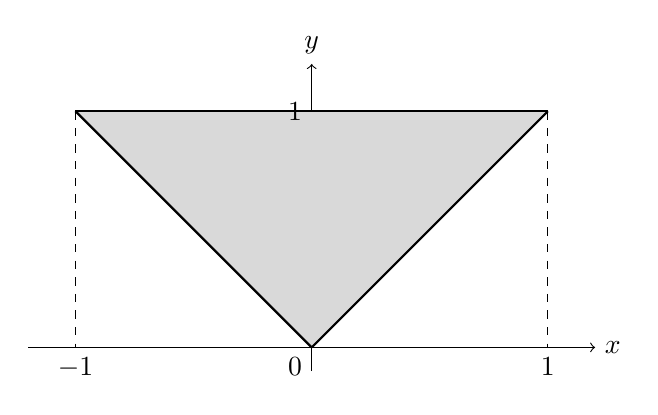
\begin{tikzpicture}[scale=3]
  \draw[->] (-1.2,0) -- (1.2,0) node[right] {$x$};
  \draw[->] (0,-0.1) -- (0,1.2) node[above] {$y$};
  \fill[gray!30] (0,0) -- (1,1) -- (-1,1) -- cycle;
  \draw[dashed] (1,1) -- (1,0) node[below] {$1$};
  \draw[dashed] (-1,1) -- (-1,0) node[below] {$-1$};
  \draw (0,1) node[left] {$1$};
  \draw[thick] (0,0) -- (1,1);
  \draw[thick] (0,0) -- (-1,1);
  \draw[thick] (-1,1) -- (1,1);
  \draw (0,0) node[below left] {$0$};
\end{tikzpicture}
\caption{Support of $(X,Y)$ for Example 3.}
\label{fig:ex3}
\end{figure}
The total probability must integrate to 1:
$$\int_{0}^{1} \int_{-y}^{y} Ky(y-x) \,dx \,dy = 1$$
Evaluating the inner integral:
\begin{align*}
\int_{-y}^{y} Ky(y-x) \,dx &= Ky \left[ yx - \frac{x^2}{2} \right]_{-y}^{y} \\
&= Ky \left( \left(y^2 - \frac{y^2}{2}\right) - \left(-y^2 - \frac{y^2}{2}\right) \right) \\
&= Ky \left( \frac{y^2}{2} - \left(-\frac{3y^2}{2}\right) \right) = Ky (2y^2) = 2Ky^3
\end{align*}
Now, integrating with respect to $y$:
$$\int_{0}^{1} 2Ky^3 \,dy = 2K \left[ \frac{y^4}{4} \right]_{0}^{1} = \frac{K}{2}$$
Equating to 1 gives $\frac{K}{2} = 1$, so $K = 2$.

\vspace{1em}

\textbf{EXAMPLE 4.} If $X$ and $Y$ have the joint probability density function
$$
f(x,y) = \begin{cases} \frac{K(1+x+y)}{(1+x)^4 (1+y)^4} & \text{if } x > 0, y > 0 \\ 0 & \text{otherwise} \end{cases}
$$
find the value of $K$.

\textbf{Solution.} For $f(x,y)$ to be a valid pdf, its integral over the support must be 1:
$$\int_{0}^{\infty} \int_{0}^{\infty} \frac{K(1+x+y)}{(1+x)^4 (1+y)^4} \,dx \,dy = 1$$
We can split the numerator $1+x+y$ into $(1+x) + y$:
\begin{align*}
\int_{0}^{\infty} \int_{0}^{\infty} & K \left( \frac{1}{(1+x)^3(1+y)^4} + \frac{y}{(1+x)^4(1+y)^4} \right) \,dx \,dy \\
&= K \int_{0}^{\infty} \frac{1}{(1+y)^4} \left[ \frac{-1}{2(1+x)^2} \right]_{0}^{\infty} dy + K \int_{0}^{\infty} \frac{y}{(1+y)^4} \left[ \frac{-1}{3(1+x)^3} \right]_{0}^{\infty} dy \\
&= K \int_{0}^{\infty} \frac{1/2}{(1+y)^4} \,dy + K \int_{0}^{\infty} \frac{y/3}{(1+y)^4} \,dy
\end{align*}
Evaluating the $y$ integrals:
$$\int_{0}^{\infty} \frac{1/2}{(1+y)^4} \,dy = \frac{1}{2} \left[ \frac{-1}{3(1+y)^3} \right]_{0}^{\infty} = \frac{1}{6}$$
$$\int_{0}^{\infty} \frac{y/3}{(1+y)^4} \,dy = \frac{1}{3} \int_{0}^{\infty} \left( \frac{1}{(1+y)^3} - \frac{1}{(1+y)^4} \right) \,dy = \frac{1}{3} \left( \frac{1}{2} - \frac{1}{3} \right) = \frac{1}{18}$$
Summing these gives:
$$K \left( \frac{1}{6} + \frac{1}{18} \right) = K \left( \frac{4}{18} \right) = \frac{2K}{9} = 1 \implies K = \frac{9}{2}$$

\vspace{1em}

\textbf{EXAMPLE 5.} If $X$ and $Y$ have the joint probability density function
$$
f(x, y) = \begin{cases} K(x+2y) & \text{if } 0 < x < 2, 0 < y < 1 \\ 0 & \text{otherwise} \end{cases}
$$
find the value of $K$.

\textbf{Solution.} The integral of the pdf over the given domain must equal 1:
\begin{align*}
\int_{0}^{1} \int_{0}^{2} K(x+2y) \,dx \,dy &= K \int_{0}^{1} \left[ \frac{x^2}{2} + 2xy \right]_{x=0}^{2} \,dy \\
&= K \int_{0}^{1} (2 + 4y) \,dy \\
&= K \left[ 2y + 2y^2 \right]_{0}^{1} \\
&= K(2 + 2) = 4K
\end{align*}
Equating to 1 gives $4K = 1 \implies K = \frac{1}{4}$.

\vspace{1em}

\textbf{EXAMPLE 6.} If $X$ and $Y$ have the joint probability density function
$$
f(x, y) = \begin{cases} K(x+y) & \text{if } 0 < x < 2, 0 < y < 2 \\ 0 & \text{otherwise} \end{cases}
$$
find (a) the value of $K$ and (b) $P(X +Y < 1)$.

\textbf{Solution.} 
(a) To find $K$:
\begin{align*}
\int_{0}^{2} \int_{0}^{2} K(x+y) \,dx \,dy &= K \int_{0}^{2} \left[ \frac{x^2}{2} + xy \right]_{x=0}^{2} \,dy \\
&= K \int_{0}^{2} (2 + 2y) \,dy = K \left[ 2y + y^2 \right]_{0}^{2} = K(4+4) = 8K
\end{align*}
Thus, $8K = 1 \implies K = \frac{1}{8}$.

(b) The region $X+Y<1$ inside the square $[0,2]\times[0,2]$ is shown in Figure~\ref{fig:ex6b}.
\begin{figure}[H]
\centering
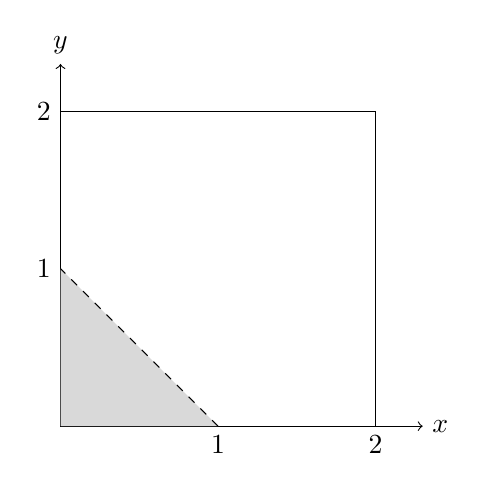
\begin{tikzpicture}[scale=2]
  \draw[->] (0,0) -- (2.3,0) node[right] {$x$};
  \draw[->] (0,0) -- (0,2.3) node[above] {$y$};
  \draw (0,0) rectangle (2,2);
  \fill[gray!30] (0,0) -- (1,0) -- (0,1) -- cycle;
  \draw[dashed] (1,0) -- (0,1);
  \draw (1,0) node[below] {$1$};
  \draw (0,1) node[left] {$1$};
  \draw (2,0) node[below] {$2$};
  \draw (0,2) node[left] {$2$};
\end{tikzpicture}
\caption{Shaded region: $X+Y<1$ for Example 6(b).}
\label{fig:ex6b}
\end{figure}
To find $P(X+Y < 1)$:
\begin{align*}
P(X+Y < 1) &= \int_{0}^{1} \int_{0}^{1-x} \frac{1}{8}(x+y) \,dy \,dx \\
&= \frac{1}{8} \int_{0}^{1} \left[ xy + \frac{y^2}{2} \right]_{y=0}^{1-x} \,dx \\
&= \frac{1}{8} \int_{0}^{1} \left( x(1-x) + \frac{(1-x)^2}{2} \right) \,dx \\
&= \frac{1}{8} \int_{0}^{1} \left( \frac{1}{2} - \frac{x^2}{2} \right) \,dx = \frac{1}{16} \left[ x - \frac{x^3}{3} \right]_{0}^{1} = \frac{1}{16} \left( \frac{2}{3} \right) = \frac{1}{24}
\end{align*}

\vspace{1em}

\textbf{EXAMPLE 7.} If the joint probability density function of $(X,Y)$ is given by
$$
f(x, y) = \begin{cases} 2e^{-x-2y} & \text{if } x > 0, y > 0 \\ 0 & \text{otherwise} \end{cases}
$$
find $P(X +Y < 1)$.

\textbf{Solution.} The region of integration is the triangle bounded by $x=0$, $y=0$, and $x+y=1$ (see Figure~\ref{fig:ex7}).
\begin{figure}[H]
\centering
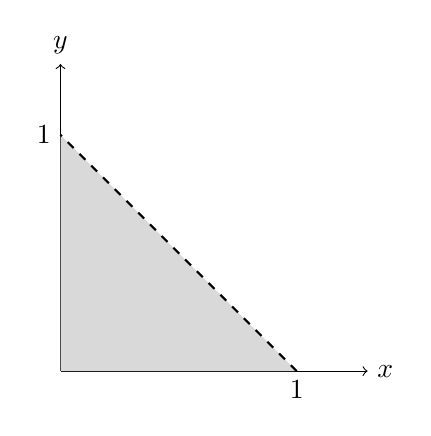
\begin{tikzpicture}[scale=3]
  \draw[->] (0,0) -- (1.3,0) node[right] {$x$};
  \draw[->] (0,0) -- (0,1.3) node[above] {$y$};
  \fill[gray!30] (0,0) -- (1,0) -- (0,1) -- cycle;
  \draw[dashed, thick] (1,0) -- (0,1);
  \draw (1,0) node[below] {$1$};
  \draw (0,1) node[left] {$1$};
\end{tikzpicture}
\caption{Shaded region: $X+Y<1$, $x>0$, $y>0$ for Example 7.}
\label{fig:ex7}
\end{figure}
\begin{align*}
P(X+Y < 1) &= \int_{0}^{1} \int_{0}^{1-x} 2e^{-x-2y} \,dy \,dx \\
&= \int_{0}^{1} 2e^{-x} \left[ \frac{-1}{2} e^{-2y} \right]_{0}^{1-x} \,dx \\
&= \int_{0}^{1} e^{-x} (1 - e^{-2(1-x)}) \,dx \\
&= \int_{0}^{1} (e^{-x} - e^{x-2}) \,dx \\
&= \left[ -e^{-x} - e^{x-2} \right]_{0}^{1} \\
&= (-e^{-1} - e^{-1}) - (-1 - e^{-2}) = 1 + e^{-2} - 2e^{-1}
\end{align*}

\vspace{1em}

\textbf{EXAMPLE 8.} If the joint probability density function of $(X,Y)$ is given by
$$
f(x, y) = \begin{cases} 6x^2y & \text{if } 0 < x < 1, 0 < y < 1 \\ 0 & \text{otherwise} \end{cases}
$$
find $P(Y > X)$.

\textbf{Solution.} The region where $Y > X$ in the unit square is the triangle above the diagonal (Figure~\ref{fig:ex8}).
\begin{figure}[H]
\centering
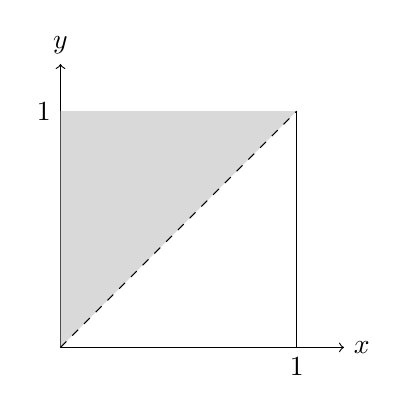
\begin{tikzpicture}[scale=3]
  \draw[->] (0,0) -- (1.2,0) node[right] {$x$};
  \draw[->] (0,0) -- (0,1.2) node[above] {$y$};
  \draw (0,0) rectangle (1,1);
  \fill[gray!30] (0,0) -- (1,1) -- (0,1) -- cycle;
  \draw[dashed] (0,0) -- (1,1);
  \draw (1,0) node[below] {$1$};
  \draw (0,1) node[left] {$1$};
\end{tikzpicture}
\caption{Shaded region: $Y>X$ for Example 8.}
\label{fig:ex8}
\end{figure}
\begin{align*}
P(Y > X) &= \int_{0}^{1} \int_{x}^{1} 6x^2y \,dy \,dx \\
&= \int_{0}^{1} 6x^2 \left[ \frac{y^2}{2} \right]_{x}^{1} \,dx \\
&= \int_{0}^{1} 3x^2 (1 - x^2) \,dx \\
&= \int_{0}^{1} (3x^2 - 3x^4) \,dx = \left[ x^3 - \frac{3x^5}{5} \right]_{0}^{1} = 1 - \frac{3}{5} = \frac{2}{5}
\end{align*}

\vspace{1em}

\textbf{EXAMPLE 9.} If the joint probability density function of $(X,Y)$ is given by
$$
f(x, y) = \begin{cases} \frac{y}{2}(1+x) & \text{if } 0 < x < 2, 0 < y < 1 \\ 0 & \text{otherwise} \end{cases}
$$
find $P(X +Y > 1)$.

\textbf{Solution.} The region $X+Y>1$ inside the rectangle $[0,2]\times[0,1]$ is shown in Figure~\ref{fig:ex9}.
\begin{figure}[H]
\centering
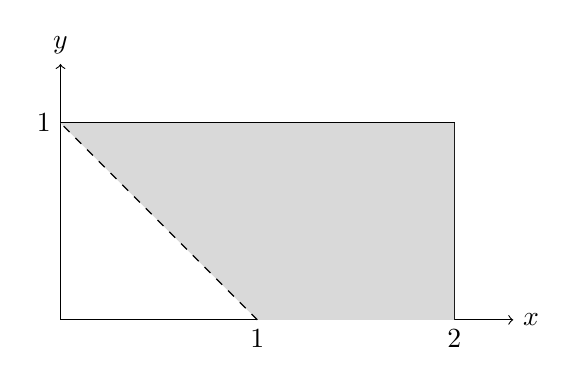
\begin{tikzpicture}[scale=2.5]
  \draw[->] (0,0) -- (2.3,0) node[right] {$x$};
  \draw[->] (0,0) -- (0,1.3) node[above] {$y$};
  \draw (0,0) rectangle (2,1);
  \fill[gray!30] (1,0) -- (2,0) -- (2,1) -- (0,1) -- cycle;
  \draw[dashed] (1,0) -- (0,1);
  \draw (1,0) node[below] {$1$};
  \draw (2,0) node[below] {$2$};
  \draw (0,1) node[left] {$1$};
\end{tikzpicture}
\caption{Shaded region: $X+Y>1$ for Example 9.}
\label{fig:ex9}
\end{figure}
We first calculate $P(X+Y < 1)$, the unshaded triangle:
\begin{align*}
P(X+Y < 1) &= \int_{0}^{1} \int_{0}^{1-y} \frac{y}{2}(1+x) \,dx \,dy \\
&= \int_{0}^{1} \frac{y}{2} \left[ x + \frac{x^2}{2} \right]_{0}^{1-y} \,dy \\
&= \int_{0}^{1} \frac{y}{2} \left( (1-y) + \frac{(1-y)^2}{2} \right) \,dy \\
&= \int_{0}^{1} \frac{y}{2} \left( \frac{3}{2} - 2y + \frac{y^2}{2} \right) \,dy \\
&= \int_{0}^{1} \left( \frac{3y}{4} - y^2 + \frac{y^3}{4} \right) \,dy \\
&= \left[ \frac{3y^2}{8} - \frac{y^3}{3} + \frac{y^4}{16} \right]_{0}^{1} = \frac{3}{8} - \frac{1}{3} + \frac{1}{16} = \frac{5}{48}
\end{align*}
Therefore, $P(X+Y > 1) = 1 - P(X+Y < 1) = 1 - \frac{5}{48} = \frac{43}{48}$.

\vspace{1em}

\textbf{EXAMPLE 10.} If the joint probability density function of $(X,Y)$ is given by
$$
f(x, y) = \begin{cases} 12e^{-3x-4y} & \text{if } x > 0, y > 0 \\ 0 & \text{otherwise} \end{cases}
$$
find (a) $P(1 < X < 3, 2 < Y < 4)$, (b) $P(X < 2, Y < 2)$ and (c) $P(X +Y < 1)$.

\textbf{Solution.} Note that $X$ and $Y$ are independent, with marginals $f_X(x) = 3e^{-3x}$ and $f_Y(y) = 4e^{-4y}$.
(a)
\begin{align*}
P(1 < X < 3, 2 < Y < 4) &= \left( \int_{1}^{3} 3e^{-3x} \,dx \right) \left( \int_{2}^{4} 4e^{-4y} \,dy \right) \\
&= \left[ -e^{-3x} \right]_{1}^{3} \left[ -e^{-4y} \right]_{2}^{4} = (e^{-3} - e^{-9})(e^{-8} - e^{-16})
\end{align*}

(b) 
\begin{align*}
P(X < 2, Y < 2) &= \left( \int_{0}^{2} 3e^{-3x} \,dx \right) \left( \int_{0}^{2} 4e^{-4y} \,dy \right) \\
&= (1 - e^{-6})(1 - e^{-8})
\end{align*}

(c) The region $X+Y<1$ is the same triangle as in Example 7 (Figure~\ref{fig:ex10c}).
\begin{figure}[H]
\centering
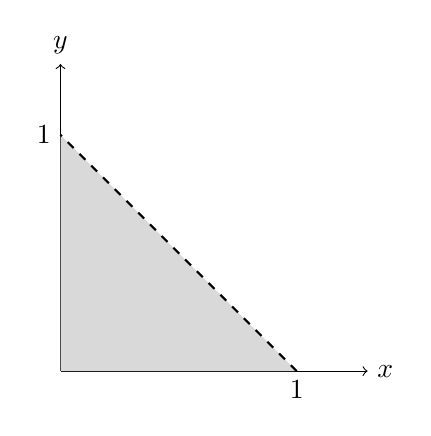
\begin{tikzpicture}[scale=3]
  \draw[->] (0,0) -- (1.3,0) node[right] {$x$};
  \draw[->] (0,0) -- (0,1.3) node[above] {$y$};
  \fill[gray!30] (0,0) -- (1,0) -- (0,1) -- cycle;
  \draw[dashed, thick] (1,0) -- (0,1);
  \draw (1,0) node[below] {$1$};
  \draw (0,1) node[left] {$1$};
\end{tikzpicture}
\caption{Shaded region: $X+Y<1$ for Example 10(c).}
\label{fig:ex10c}
\end{figure}
\begin{align*}
P(X+Y < 1) &= \int_{0}^{1} \int_{0}^{1-x} 12e^{-3x-4y} \,dy \,dx \\
&= \int_{0}^{1} 3e^{-3x} \left[ -e^{-4y} \right]_{0}^{1-x} \,dx \\
&= \int_{0}^{1} 3e^{-3x} (1 - e^{-4(1-x)}) \,dx = 3 \int_{0}^{1} (e^{-3x} - e^{x-4}) \,dx \\
&= 3 \left[ \frac{-e^{-3x}}{3} - e^{x-4} \right]_{0}^{1} = \left[ -e^{-3x} - 3e^{x-4} \right]_{0}^{1} \\
&= (-e^{-3} - 3e^{-3}) - (-1 - 3e^{-4}) = 1 + 3e^{-4} - 4e^{-3}
\end{align*}

\vspace{1em}

\textbf{EXAMPLE 11.} If the joint probability density function of $(X,Y)$ is given by
$$
f(x, y) = \begin{cases} 1 & \text{if } 0 < x < 1, 0 < y < 1 \\ 0 & \text{otherwise} \end{cases}
$$
find (a) $P(X < \frac{1}{2}, Y > \frac{1}{2})$ and (b) $P(X +Y < \frac{1}{2})$.

\textbf{Solution.}
(a) The region is a rectangle of width $1/2$ and height $1/2$ (Figure~\ref{fig:ex11a}).
\begin{figure}[H]
\centering
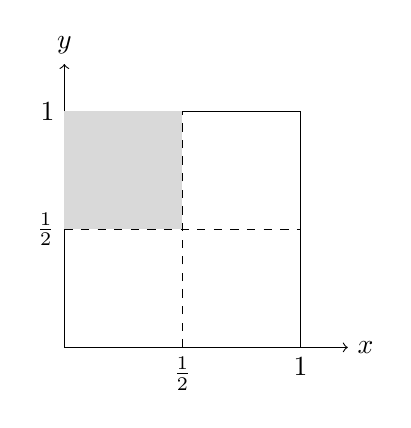
\begin{tikzpicture}[scale=3]
  \draw[->] (0,0) -- (1.2,0) node[right] {$x$};
  \draw[->] (0,0) -- (0,1.2) node[above] {$y$};
  \draw (0,0) rectangle (1,1);
  \fill[gray!30] (0,0.5) rectangle (0.5,1);
  \draw[dashed] (0.5,0) -- (0.5,1);
  \draw[dashed] (0,0.5) -- (1,0.5);
  \draw (0.5,0) node[below] {$\frac{1}{2}$};
  \draw (0,0.5) node[left] {$\frac{1}{2}$};
  \draw (1,0) node[below] {$1$};
  \draw (0,1) node[left] {$1$};
\end{tikzpicture}
\caption{Shaded region for $X<\frac{1}{2}, Y>\frac{1}{2}$.}
\label{fig:ex11a}
\end{figure}
$$P\left(X < \frac{1}{2}, Y > \frac{1}{2}\right) = \int_{1/2}^{1} \int_{0}^{1/2} 1 \,dx \,dy = \frac{1}{2} \times \frac{1}{2} = \frac{1}{4}$$

(b) The region is a triangle with vertices $(0,0)$, $(1/2,0)$, and $(0,1/2)$ (Figure~\ref{fig:ex11b}).
\begin{figure}[H]
\centering
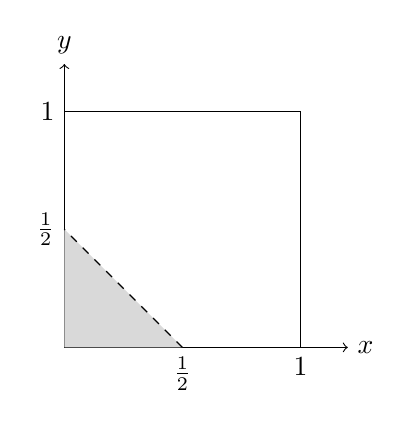
\begin{tikzpicture}[scale=3]
  \draw[->] (0,0) -- (1.2,0) node[right] {$x$};
  \draw[->] (0,0) -- (0,1.2) node[above] {$y$};
  \draw (0,0) rectangle (1,1);
  \fill[gray!30] (0,0) -- (0.5,0) -- (0,0.5) -- cycle;
  \draw[dashed] (0.5,0) -- (0,0.5);
  \draw (0.5,0) node[below] {$\frac{1}{2}$};
  \draw (0,0.5) node[left] {$\frac{1}{2}$};
  \draw (1,0) node[below] {$1$};
  \draw (0,1) node[left] {$1$};
\end{tikzpicture}
\caption{Shaded region for $X+Y<\frac{1}{2}$.}
\label{fig:ex11b}
\end{figure}
$$P\left(X +Y < \frac{1}{2}\right) = \int_{0}^{1/2} \int_{0}^{1/2-x} 1 \,dy \,dx = \frac{1}{2} \left(\frac{1}{2}\right) \left(\frac{1}{2}\right) = \frac{1}{8}$$

\vspace{1em}

\textbf{EXAMPLE 12.} If the joint probability density function of $(X,Y)$ is given by
$$
f(x,y) = \begin{cases} 2 & \text{if } x > 0, y > 0, x+y < 1 \\ 0 & \text{otherwise} \end{cases}
$$
find (a) $P(X < \frac{1}{2}, Y < \frac{1}{2})$, (b) $P(X +Y < \frac{1}{2})$, and (c) $P(X > 2Y)$.

\textbf{Solution.} The support is the triangle bounded by $x=0$, $y=0$, and $x+y=1$. The regions for each part are shown in Figure~\ref{fig:ex12}.
\begin{figure}[H]
\centering
\begin{subfigure}[b]{0.3\textwidth}
\centering
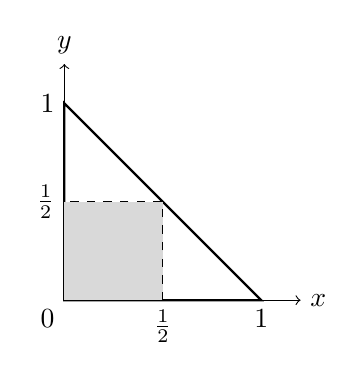
\begin{tikzpicture}[scale=2.5]
  \draw[->] (0,0) -- (1.2,0) node[right] {$x$};
  \draw[->] (0,0) -- (0,1.2) node[above] {$y$};
  \draw[thick] (0,1) -- (1,0) -- (0,0) -- cycle;
  \fill[gray!30] (0,0) rectangle (0.5,0.5);
  \draw[dashed] (0.5,0) -- (0.5,0.5) -- (0,0.5);
  \draw (0.5,0) node[below] {$\frac{1}{2}$};
  \draw (0,0.5) node[left] {$\frac{1}{2}$};
  \draw (1,0) node[below] {$1$};
  \draw (0,1) node[left] {$1$};
  \draw (0,0) node[below left] {$0$};
\end{tikzpicture}
\caption{Region for $X<\frac{1}{2}, Y<\frac{1}{2}$}
\end{subfigure}
\hfill
\begin{subfigure}[b]{0.3\textwidth}
\centering
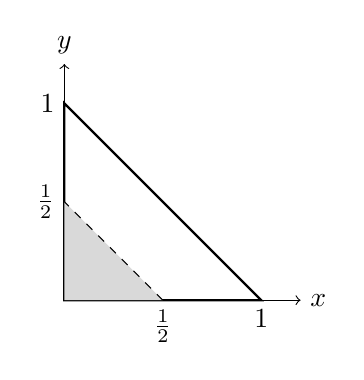
\begin{tikzpicture}[scale=2.5]
  \draw[->] (0,0) -- (1.2,0) node[right] {$x$};
  \draw[->] (0,0) -- (0,1.2) node[above] {$y$};
  \draw[thick] (0,1) -- (1,0) -- (0,0) -- cycle;
  \fill[gray!30] (0,0) -- (0.5,0) -- (0,0.5) -- cycle;
  \draw[dashed] (0.5,0) -- (0,0.5);
  \draw (0.5,0) node[below] {$\frac{1}{2}$};
  \draw (0,0.5) node[left] {$\frac{1}{2}$};
  \draw (1,0) node[below] {$1$};
  \draw (0,1) node[left] {$1$};
\end{tikzpicture}
\caption{Region for $X+Y<\frac{1}{2}$}
\end{subfigure}
\hfill
\begin{subfigure}[b]{0.3\textwidth}
\centering
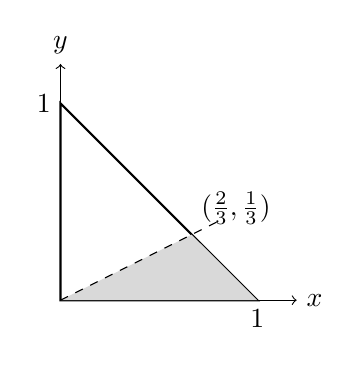
\begin{tikzpicture}[scale=2.5]
  \draw[->] (0,0) -- (1.2,0) node[right] {$x$};
  \draw[->] (0,0) -- (0,1.2) node[above] {$y$};
  \draw[thick] (0,1) -- (1,0) -- (0,0) -- cycle;
  \fill[gray!30] (0,0) -- (1,0) -- (0.666,0.333) -- cycle;
  \draw[dashed] (0,0) -- (0.8,0.4);
  \draw (1,0) node[below] {$1$};
  \draw (0,1) node[left] {$1$};
  \draw (0.666,0.333) node[above right] {$(\frac{2}{3},\frac{1}{3})$};
\end{tikzpicture}
\caption{Region for $X>2Y$}
\end{subfigure}
\caption{Shaded regions for Example 12.}
\label{fig:ex12}
\end{figure}

(a) The region is a square entirely contained within the support $x+y < 1$.
$$P\left(X < \frac{1}{2}, Y < \frac{1}{2}\right) = \int_{0}^{1/2} \int_{0}^{1/2} 2 \,dx \,dy = 2 \left(\frac{1}{4}\right) = \frac{1}{2}$$

(b) The region is a smaller triangle.
$$P\left(X +Y < \frac{1}{2}\right) = \int_{0}^{1/2} \int_{0}^{1/2-x} 2 \,dy \,dx = 2 \left[ \frac{1}{2} \left(\frac{1}{2}\right) \left(\frac{1}{2}\right) \right] = \frac{1}{4}$$

(c) The line $X=2Y$ intersects the boundary $X+Y=1$ at $(2/3, 1/3)$.
\begin{align*}
P(X > 2Y) &= \int_{0}^{1/3} \int_{2y}^{1-y} 2 \,dx \,dy \\
&= \int_{0}^{1/3} 2(1 - y - 2y) \,dy = \int_{0}^{1/3} (2 - 6y) \,dy \\
&= \left[ 2y - 3y^2 \right]_{0}^{1/3} = 2\left(\frac{1}{3}\right) - 3\left(\frac{1}{9}\right) = \frac{2}{3} - \frac{1}{3} = \frac{1}{3}
\end{align*}

\end{document}